\documentclass[a4paper,12pt]{article}

\usepackage[utf8]{inputenc}
\usepackage[T1]{fontenc}
\usepackage[brazil]{babel}
\usepackage{fancyhdr}
\usepackage{graphicx}
\usepackage{float}
\pagestyle{fancy}
\setlength{\headheight}{14.49998pt}
\fancyhf{}

\title{Game Design Document}
\author{
    Henrique Finatti Silveira Belo Trebbi \\
    Tiago Fagundes dos Santos \\
    Mateus Marana Assuena \\
    Giovanni Chahin Morassi \\
}
\date{Março de 2026}

\renewcommand{\headrulewidth}{0.5pt}
\fancyhead[L]{FeiKemon}
\fancyhead[R]{CC7140 - Jogos Digitais}

\renewcommand{\footrulewidth}{0.5pt}
\fancyfoot[L]{FeiKemon}
\fancyfoot[C]{\thepage}
\fancyfoot[R]{FEI - SBC}

\begin{document}

\maketitle
\newpage
\tableofcontents

\newpage
\section{Página de Título}
\subsection{Título do Jogo}
FeiKemon

\subsection{Sistemas do Jogo}
\subsubsection{Movimentação no mapa}
O jogador poderá explorar o mapa utilizando os botões de movimentação “A”, “W”, “S” e “D”.

\subsubsection{Interações com os NPCs}
O jogador poderá interagir com os NPCs do mapa chegando perto o bastante e clicando com a barra de espaço.
Um som será emitido quando essa interação ocorrer.

\subsubsection{Combate}
Quando uma batalha começa, seja contra um NPC ou com um FeiKemon aleatório,
o jogador pode utilizar os botões de movimento para selecionar o tipo de interação.
“Atacar”, “Fugir” ou “Capturar” ou, caso tenha selecionado “Atacar”,
o jogador pode selecionar os golpes com os botões de movimento também.

\subsection{Faixa etária recomendada dos jogadores}
O jogo é recomendado para jogadores que estão ingressando na faculdade,
por tanto a faixa etária recomendada é entre +17.

\subsection{Classificação indicativa ESRB pretendida}
T (Teen). Pode conter violência, temas sugestivos, humor grosseiro, mínimo sangue e uso ocasional de linguagem forte.

\subsection{Data de lançamento prevista}
A data de lançamento prevista é 11/05/2026.

\newpage
\section{Esboço do Jogo}
\subsection{História do jogo}
O jogo é um jogo top-down, visto de cima, que se passa no dia da recepção dos calouros da faculdade FEI, e tem como personagem principal
um ansioso garoto que acaba de se matricular na sua faculdade dos sonhos, com o objetivo se tornar um especialista em computação e seguir os passos da família
em estudar na FEI.

Durante a recepção o aluno terá uma palestra da reitoria onde irá conhecer algumas curiosidades sobre a faculdade e os FeiKemons,
após isso será convidado a conhecer a faculdade e os prédios dos cursos disponíveis. Durante sua exploração o jogador irá perceber que
há algo estranho com a faculdade e que só ele e o professor Fagner percebem isso, o aluno irá mais a fundo na história para descobrir que a faculdade
Mauá está impactando negativamente a faculdade e ele deve salva-la.

Para salva-la o aluno irá montar um time de FeiKemons e derrotar os mestres da FEI para remover os efeitos da Mauá, mas para isso ele precisa primeiro derrotar
a chefe de departamento de computação para conseguir acesso a sala dos mestres.
Os mestres da FEI são a reitoria, o padre e professor Samir.

\subsection{Fluxo do Jogo}
O jogador irá experiênciar a história e a faculdade como o ansioso rapaz determinado a conhecer a faculdade, ele será surpreendido por
alguns desafios durante a história e precisará de uma equipe de FeiKemons para passar por eles, sendo necessário evoluir essa equipe com o tempo
para se manter preparado para os desafios seguintes.

Conforme o jogador vence batalhas ele adquiri conhecimentos e isso deixa seus FeiKemons mais fortes. Conforme o jogador vence treinadores
ele também receberá acessos para outras partes do jogo, a fim de garantir o fluxo correto da história.

O jogador será vitorioso quando conseguir derrotar os mestres da FEI e salvar as mentes da FEI das garras da faculdade Mauá.

\newpage
\section{Personagens}
\subsection{Personagem Principal}
O personagem principal tem uma breve história, ele é o mais novo membro de uma familia onde todos estudaram na FEI e sonha com isso desde que pode entender o que isso significa.
Pelas histórias que ouvia de seus familiares sobre a FEI ele percebeu uma diferença muito grande do que ouvia para o que vê na faculdade,
isso gerou uma estranheza e com o estímulo e ajuda do Fagner ele descobriu que a faculdade está sobre os efeitos da Mauá.


As principais teclas do jogador serão as teclas A, W, S, D e a Barra de espaço, onde a ação de cada uma delas pode variar com
o contexto que estão sendo usadas.
\begin{figure}[H]
    \centering
    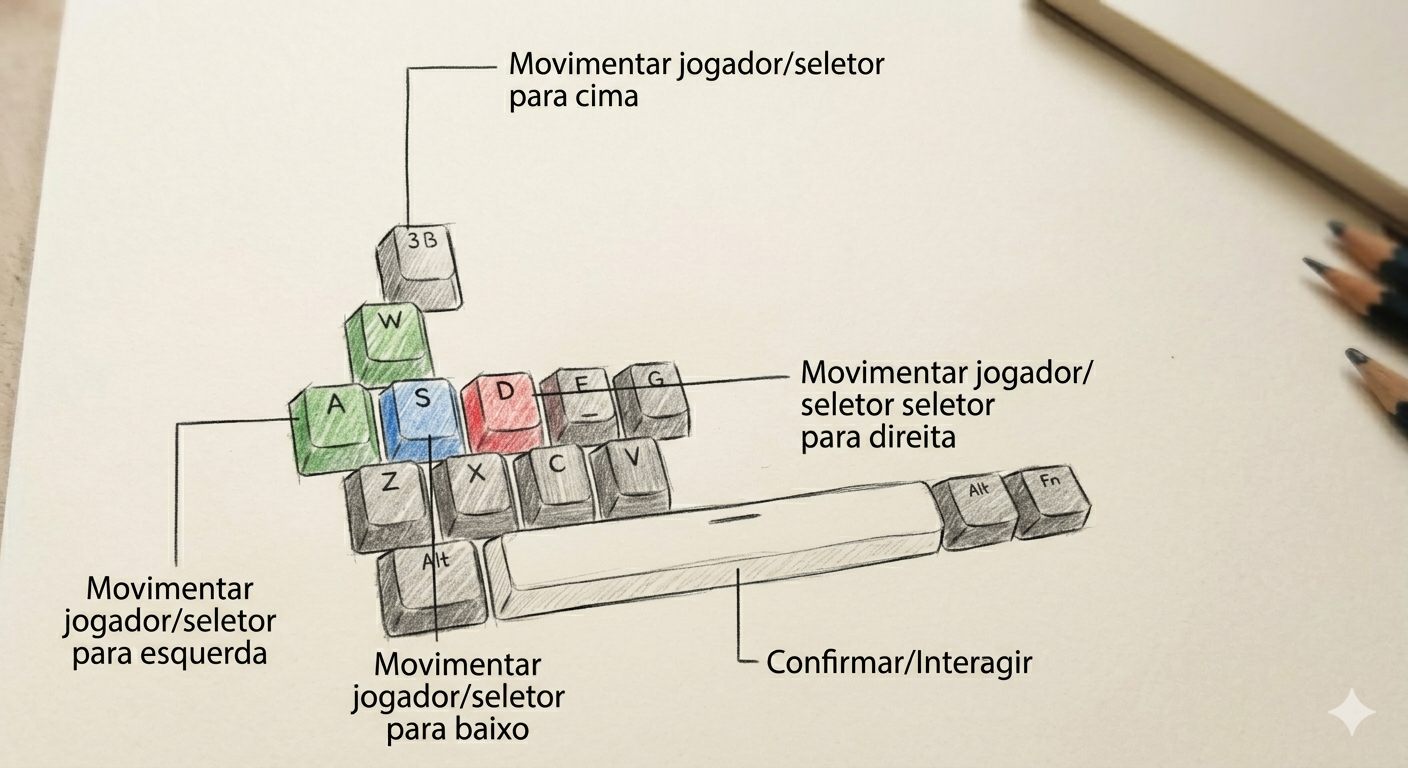
\includegraphics[width=0.8\textwidth]{MapaDeControles.png}
    \caption{Mapa de controles do jogador.}
    \label{fig:meu_grafico}
\end{figure}

\subsection{FeiKemons}
Esses, com certeza são os personagens mais frequentes do jogo, são pequenos monstrinhos que representam matérias do curso de computação
ou itens relacionados ao curso como os sistemas operacionais, computadores, mas isso não reflete apenas nos visuais, cada FeiKemon terá suas tipagens, 
as tipagens, as tipagens serão as matérias apresentadas no curso de Computação.
Cada FeiKemon poderá ser capturado pelo jogador, uma vez capturado o jogador pode usar esse FeiKemon em batalhas e aumentar o nível deles, 
o quão mais alto for o nível mais forte o FeiKemon será.

\subsection{Outros personagens presentes no jogo}
\begin{itemize}
    \item Professor Fagner (Único professor fora dos efeitos da Mauá);
    \item Professora Leila (Chefe de departamento e primeiro boss do jogo);
    \item Professor Samir (Membro dos mestres da FEI)
    \item Reitoria (Membro dos mestres da FEI)
    \item Padre (Membro dos mestres da FEI)
\end{itemize}
\subsubsection{Professor Fagner}
Esse é o único professor da FEI que sente que algo de errado está acontecendo na faculdade e te dá todo suporte durante a jornada.

\subsubsection{Professora Leila}
Essa é a chefe de departamento, a professora mais forte do departamento de computação. O jogador deverá derrota-la primeiro
antes de poder enfrentar os mestres da FEI.

\subsubsection{Professor Samir}
O último professor a ser enfrentado e o mais forte também, ele estará disponívei apenas uma vez durante a batalha contra os mestres da FEI 
e terá a FeiKemons do tipo matemática.

\subsubsection{Refeitora}
Será um único treinador representando a reitoria da FEI e será o primeiro dos mestres da FEI.

\subsubsection{Padre}
O segundo mestre da FEI e terá FeiKemons que representam o início da FEI.

\newpage
\section{Gameplay}

O jogo é um JRPG com camêra top-down e totalmente single player, a gameplay foca no treinamento e montagem de um time de FeiKemons para progredir
a história, a história será separada em pequenos capitulos, sem uma transição explicita entre um e outro.

O jogo terá cenários que lembram a estrutura da faculdade FEI, porém os sprites serão baseados no jogo Stardew Valley, por tanto
alguns cenários irão sofrer com a falta de detalhes da faculdade.

O jogo também contará com efeitos sonoros e músicas que refletem as situações que jogador está vivenciando para enriquecer a gameplay.

\newpage
\section{Mundo Do Jogo}
O do jogo reflete alguns cenários da faculdade FEI, dentro os inúmeros cenários da FEI, somente alguns serão acessíveis ao
jogador, sendo eles a sala de estudos, o estacionamento dos professores, a capela, o prédio K, o MacFEI de cima e a entrada da FEI.

Esses cenários serão acessados como diferentes mapas e terão uma transição de cena entre eles.
\subsection{Cenários e a História}
Dentro de todos os cenários apresentados no jogo alguns estarão disponíveis para certas etapas da história, e cada um terá sua
devida funcionalidade para o jogador.

\subsubsection{Entrada da FEI}
Será o ponto de início do jogo e onde o jogador poderá começar a movimentar o jogador, essa área do jogo poderá ser acessada a qualquer etapa da história
porém só terá obrigatoriedade no inicio do jogo.

\subsubsection{Sala de estudos}
Aqui a história começará a tomar forma, será aqui que o jogador entrará em contato com os primeiros personagens da história e onde receberá a primeira missão,
de explorar a faculdade. Também será uma área que poderá ser acessada a qualquer momento, mas só terá relevância para a história duas vezes.

\subsubsection{Estacionamento dos professores}
É apenas uma área que serve para interligar a sala de estudos com outras áreas do jogo, não tem relevância para a história.

\subsubsection{Capela}
A capela será onde o jogador irá lutar contra os mestres da FEI, será possível acessar essa área apenas para a luta final.

\subsubsection{Prédio K}
Será o local onde o jogador terá a maioria das lutas e onde irá enfrentar a chefe de departamento, professora Leila.
Nessa área do jogo o jogador também conseguirá acesso a sala dos mestres da FEI.

\subsubsection{MacFEI de cima}
Será o local onde o jogador poderá recuperar seus FeiKemons, não tem relevância para a história, mas estará sempre disponível
e deve ser uma das áreas mais visitadas pelo jogador.

\newpage
\section{Experiência de Jogo}
\subsection{Tela Inicial}
O jogo, quando aberto, terá uma tela inicial com a logo do jogo e também o prédio K, um dos prédios mais emblemáticos da faculdade,
no fundo da tela, além de uma música calma, mas também misteriosa tocando, introduzindo a atmosfera do jogo ao jogador.

\subsection{Efeitos Sonoros}
O jogo terá diversos efeitos sonoros baseados nas ações do jogador ao longo da história.

\subsubsection{Musicas}
As músicas são uma parte constante do jogo, elas tocarão constantemente durante todo o jogo e irão mudar seu estilo de acordo
com a situação em que o jogador está, músicas mais calmas tocarão quando o jogador estiver parado, músicas mais intensas tocarão durante batalhas e
uma música mais misteriosa tocará quando o jogador estiver em partes mais importantes da história.

\subsubsection{Outros efeitos}
Além das músicas outros sons serão explorados para complementar a experiência do jogador, sons quando o jogador clica ou interage
com outros NPCs serão utilizados para ajudar a dar uma sensação de que a ação está sendo feita para o jogador. Além disso teremos sons
para ataques e cura de FeiKemons.

\subsection{Cenas}
Durante o jogo haverão algumas cenas que contarão parte da história, essas cenas serão importante para garantir o fluxo do Jogo
e dar a sensação que tem outras coisas acontecendo no universo do jogo enquanto ele joga. Essa cenas terão visuais semelhantes ao jogo, dando
o efeito que durante as cenas o jogo está jogando sozinho, permitindo ao jogador apenas assistir e consolidar as ações das suas últimas missões.

\newpage
\section{Mecânicas}
O jogo possui mecanicas simples, porém bem frequentes e relevantes em todo jogo. Entre essas mecânicas temos as batalhas, capturas e cura de FeiKemons.

\subsection{Batalhas}
Durante todo o jogo as batalhas serão peças chave na história, as batalhas podem ocorrer de forma aleatória ou quando um NPC te ataca.

\subsubsection{Batalhas aleatórias}
Esse tipo de batalha irá acontecer quando um FeiKemon atacar você durante o jogo, eles não são visíveis no mapa então o jogador apenas
será surpreendido por um FeiKemon aleatório o atacando. Esses ataques só acontecerão em partes externas da faculdade.

\subsubsection{Batalhas contra NPCs}
Durante o jogo haverão NPCs enfrentáveis que irão desafiar o jogador quando o jogador passar na frente deles, essas batalhas são semelhantes às
batalhas contra FeiKemons aleatórios, porém aqui o número de FeiKemons a enfrentar será maior e eles serão mais fortes também.

\subsection{Captura de FeiKemons}
FeiKemons poderão ser capturados ao longo da jornada, porém apenas os FeiKemons que não pertencem a treinadores podem ser capturados.
Para capturar um FeiKemon o jogador terá que enfraquece-lo e jogar um Feikebola nele para fazer a captura.

\subsection{Cura de FeiKemons}
FeiKemons podem perder pontos de vida durante as batalhas e será necessário curá-los frequentemente, para curá-los o jogador pode visitar o MacFEI de cima para recuperar a vida dos FEiKemons.

\newpage
\section{Inimigos}
Durante o jogo teremos alguns NPCs inimigos conhecidos, alguns desconhecidos e outros que além de conhecidos são do tipo BOSS.

\subsection{NPCs inimigos conhecidos}
Esses NPCs serão professores da FEI, que estarão sob controle da Mauá, não necessariamente tem alguma relevância para a história, mas enfrenta-los
é uma obrigatoriedade do fluxo do jogo.

\subsection{NPCs inimigos desconhecidos}
Esses NPCs serão outros alunos que serão encontrados durante o jogo, eles não tem relevância alguma para a história e servem apenas para introduzir mais batalhas ao jogador

\subsection{BOSS}
Teremos 5 BOSS, o primeiro deles será a chefe de departamento de Ciência da Computação, a professora Leila, ela estará disponível
somente após derrotar todos os outros professores da disponíveis da faculdade.
Outros 3 estarão disponíveis na sala dos mestres da FEI após a derrota da professora Leila, sendo um deles a reitoria, um deles o padre e o último o professor Samir.

Derrotando os mestres da FEI o jogador será apresentado ao mestre da Mauá que está controlando a faculdade, derrotando ele o jogador salvará a faculdade

\newpage
\section{Cenas de Corte}
O jogo contará com algumas cenas de corte e animações de transição de cena, essas cenas serão utilizadas tanto em momentos comuns quanto para contar
parte da história do jogo. Essas cenas serão desenvolvidas com a própria ferramenta de desenvolvimento do jogo, Lua e Love2D.

\subsection{Cenas de Corte da História}
Durante alguns momentos da história algumas cenas irão acontecer, essas cenas serão desenvolvidas com movimentos automáticos do jogo, dando a 
sensação para o jogador de que uma cena está acontecendo, mas sem quebrar o estilo do jogo, essas cenas serão muito mais voltadas para diálogos e 
explicações sobre a história.

\subsection{Outras Cenas}
Algumas ações no jogo podem promover outros tipos de cenas, sendo elas as cenas de cura, batalha e transição de mapas.

\subsubsection{Cenas de Cura}
As cenas de cura são apenas uma breve animação que indica que os FeiKemons estão sendo curados, essa contará com algumas músicas também.

\subsubsection{Cenas de Batalha}
Quando o jogador for desafiado para uma batalha uma breve cena irá acontecer, a tela irá piscar algumas vezes e a música irá trocar.

\subsubsection{Cenas de transição}
Essas são as cenas mais simples e acontecerão toda vez que o jogador entrar ou sair de um cenário, essas cenas contarão com o escurecimento 
da tela no mapa antigo e clareamento da tela já no cenário novo.

\newpage
\section{Material Bônus}
Sem dúvidas, o maior estímulo para o jogador jogar novamente será as diferentes combinações de times FeiKemons que o jogador pode fazer.
Cada seção será uma aventura se o tipo de equipe e estratégia for diferente.

\end{document}